\documentclass{article}
\usepackage{tikz}

\begin{document}

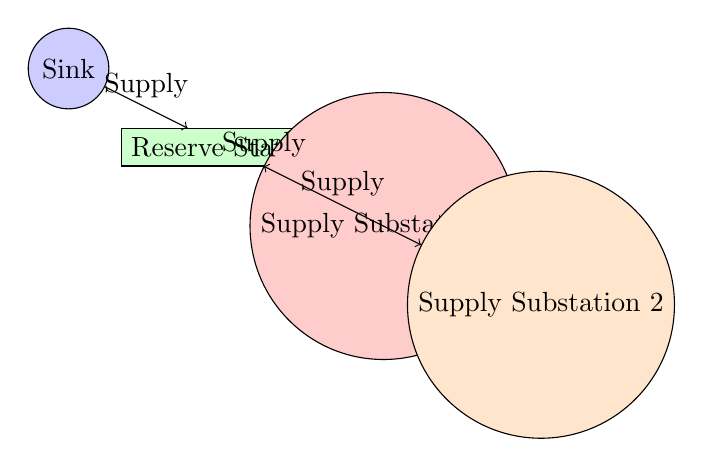
\begin{tikzpicture}[node distance=2cm]

    % Nodes for Sink, Reserve Station, and Supply Stations
    \node (sink) at (0,0) [draw, circle, fill=blue!20] {Sink};
    \node (reserve_station) at (2,-1) [draw, rectangle, fill=green!20] {Reserve Station};
    \node (supply_substation_1) at (4,-2) [draw, circle, fill=red!20] {Supply Substation 1};
    \node (supply_substation_2) at (6,-3) [draw, circle, fill=orange!20] {Supply Substation 2};

    % Drawing arrows between nodes
    \draw[->] (sink) -- node[midway, above] {Supply} (reserve_station);
    \draw[->] (reserve_station) -- node[midway, above] {Supply} (supply_substation_1);
    \draw[->] (reserve_station) -- node[midway, above] {Supply} (supply_substation_2);

\end{tikzpicture}

\end{document}